\chapter{Rectilinear Motion}
\label{ch:rectilinear}
\begin{chapterintro}
\textbf{You will learn to:} solve uniform and uniformly accelerated rectilinear
motion; handle free fall; read motion graphs; and integrate a variable
acceleration.
\end{chapterintro}

\section{Uniform rectilinear motion}

When the acceleration is zero, the velocity is constant:
\[
a=0,\qquad v=v_0,\qquad x(t)=x_0+v_0t.
\]
The $x$--$t$ graph is a straight line of slope $v_0$.

\section{Uniformly accelerated rectilinear motion}

When $a$ is constant,
\[
v(t)=v_0+at,
\]
\[
x(t)=x_0+v_0t+\frac12at^2,
\]
and, eliminating $t$,
\[
v^2-v_0^2=2a(x-x_0).
\]
The last relation is useful when time is neither given nor asked for.

\begin{figure}[htbp]
\centering
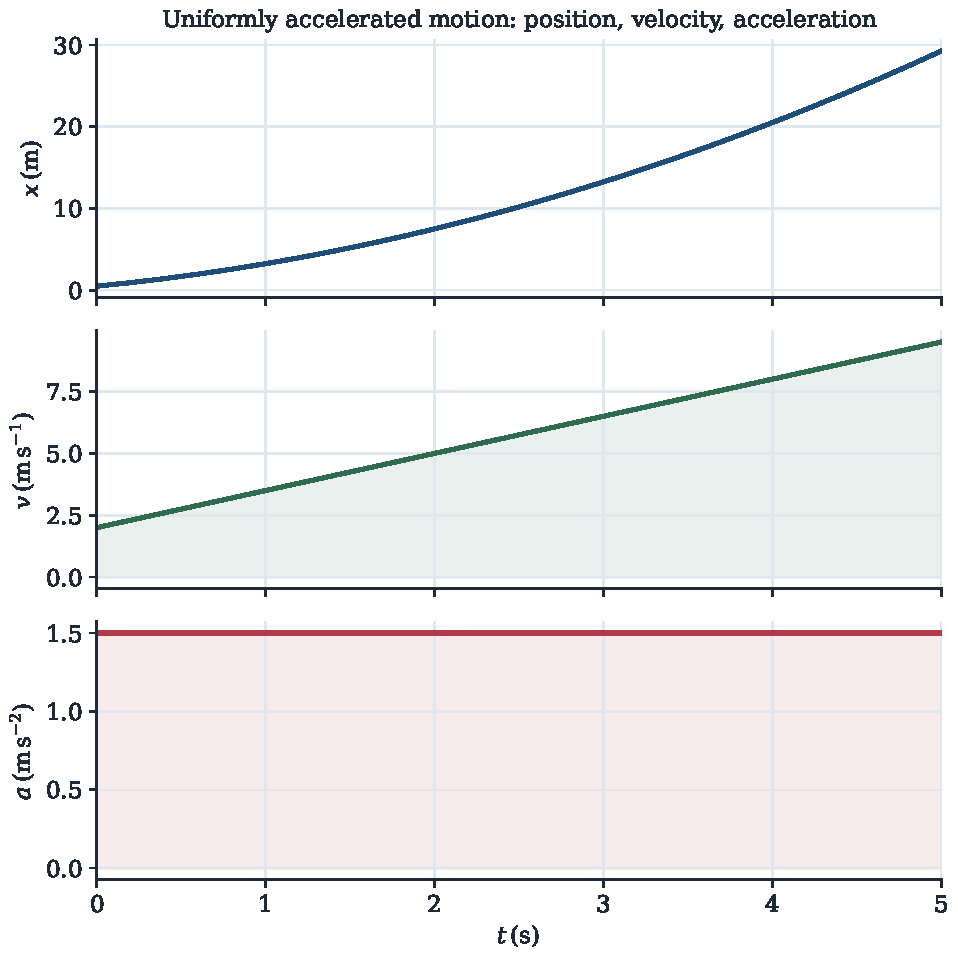
\includegraphics[width=0.78\textwidth]{figures/05_motion_graphs.pdf}
\caption{Uniformly accelerated motion with $x_0=0.5\ \mathrm{m}$,
$v_0=2.0\ \mathrm{m\,s^{-1}}$, and $a=1.5\ \mathrm{m\,s^{-2}}$. The slope of
$x(t)$ is $v(t)$; the slope of $v(t)$ is $a$; the area under $v(t)$ is the
displacement.}
\label{fig:motion-graphs}
\end{figure}

\section{Free fall}

Near the Earth's surface, neglecting air resistance, a body falls with constant
acceleration $\vec g$ directed downward. Taking the $y$-axis upward,
\[
a_y=-g,\qquad v_y=v_{0y}-gt,\qquad y=y_0+v_{0y}t-\frac12gt^2.
\]
With $g=9.81\ \mathrm{m\,s^{-2}}$.

\begin{warning}[Signs]
Choose a positive direction once and keep it for the whole problem. If upward is
positive, then $g$ enters as $-g$, a downward velocity is negative, and a
displacement below the starting point is negative.
\end{warning}

\section{Variable acceleration}

If $a$ is not constant, integrate:
\[
a(t)=\frac{\dd v}{\dd t}\implies v(t)=v(0)+\int_0^t a(t')\,\dd t',
\]
\[
v(t)=\frac{\dd x}{\dd t}\implies x(t)=x(0)+\int_0^t v(t')\,\dd t'.
\]
Two alternative forms are often useful:
\[
a=\frac{\dd v}{\dd t}=v\frac{\dd v}{\dd x}.
\]
The second form is the key to problems where the acceleration is given as a
function of position or speed.

\begin{method}[Choosing the right equation]
\begin{itemize}[leftmargin=1.3em,itemsep=2pt]
  \item Constant acceleration and time known: use $v=v_0+at$.
  \item Constant acceleration, time unknown: use $v^2=v_0^2+2a\Delta x$.
  \item Acceleration depends on $v$: separate variables in $\dd v/a(v)=\dd t$.
  \item Acceleration depends on $x$: use $v\,\dd v=a(x)\,\dd x$.
\end{itemize}
\end{method}

% ===========================================================================
\section{Worked examples}

\begin{worked}[Uniform acceleration]
A car accelerates uniformly from $10.0\ \mathrm{m\,s^{-1}}$ to
$30.0\ \mathrm{m\,s^{-1}}$ over a distance of $200\ \mathrm{m}$. Find its
acceleration and the time taken.
\end{worked}

\begin{solution}{4.1}
Use $v^2-v_0^2=2a\Delta x$:
\[
a=\frac{v^2-v_0^2}{2\Delta x}
=\frac{30.0^2-10.0^2}{2(200)}
=\frac{800}{400}=2.00\ \mathrm{m\,s^{-2}}.
\]
Then
\[
t=\frac{v-v_0}{a}=\frac{30.0-10.0}{2.00}=10.0\ \mathrm{s}.
\]
\end{solution}

\begin{worked}[Vertical throw]
A ball is thrown vertically upward from the ground with
$v_0=20.0\ \mathrm{m\,s^{-1}}$. Neglecting air resistance, find its maximum
height, the total time before it returns to the ground, and its velocity at
$t=3.00\ \mathrm{s}$.
\end{worked}

\begin{solution}{4.2}
Take upward as positive, so $a=-g=-9.81\ \mathrm{m\,s^{-2}}$.

At the highest point $v=0$:
\[
0=v_0^2-2gh
\implies
h=\frac{v_0^2}{2g}=\frac{400}{19.62}=20.4\ \mathrm{m}.
\]
The time to reach the top is $t_{\mathrm{up}}=v_0/g=2.04\ \mathrm{s}$; the total
time is twice this, $4.08\ \mathrm{s}$.

At $t=3.00\ \mathrm{s}$:
\[
v=20.0-9.81(3.00)=-9.43\ \mathrm{m\,s^{-1}}.
\]
The negative sign means the ball is moving downward.
\end{solution}

% ===========================================================================
\section{Exercises and Step-by-Step Solutions}

\begin{exercise}{\warm\ From zero to one hundred}
A car accelerates uniformly from rest to $100\ \mathrm{km\,h^{-1}}$ in
$8.00\ \mathrm{s}$. Find its acceleration and the distance covered.
\end{exercise}

\begin{tabletworkspace}[6.5cm]
\end{tabletworkspace}

\begin{solution}{4.1}
First convert:
\[
100\ \mathrm{km\,h^{-1}}=\frac{100}{3.6}=27.8\ \mathrm{m\,s^{-1}}.
\]
\[
a=\frac{v}{t}=\frac{27.8}{8.00}=3.47\ \mathrm{m\,s^{-2}}.
\]
\[
d=\frac12at^2=\frac12(3.47)(8.00)^2=111\ \mathrm{m}.
\]
Equivalently $d=v^2/(2a)=111\ \mathrm{m}$.
\end{solution}

\begin{exercise}{\warm\ Free fall}
A stone is dropped from rest from a height of $45.0\ \mathrm{m}$. Neglecting air
resistance, find the time to reach the ground and the impact speed.
\end{exercise}

\begin{tabletworkspace}[6.5cm]
\end{tabletworkspace}

\begin{solution}{4.2}
Taking downward as positive,
\[
h=\frac12gt^2
\implies
t=\sqrt{\frac{2h}{g}}=\sqrt{\frac{90.0}{9.81}}=3.03\ \mathrm{s}.
\]
\[
v=gt=9.81(3.03)=29.7\ \mathrm{m\,s^{-1}}.
\]
\end{solution}

\begin{exercise}{\warm\ Reading a position function}
A particle moves on the $x$-axis with $x(t)=3t^2-12t+7$ (SI units).
(a) Find $v(t)$ and $a(t)$.
(b) Find the time and value of the minimum position.
(c) Sketch $x(t)$ and describe the motion.
\end{exercise}

\begin{tabletworkspace}[6.5cm]
\end{tabletworkspace}

\begin{solution}{4.3}
(a)
\[
v(t)=6t-12,\qquad a(t)=6.
\]
(b) $v=0$ at $t=2.00\ \mathrm{s}$. Since $a>0$, this is a minimum:
\[
x(2)=3(4)-12(2)+7=-5.00\ \mathrm{m}.
\]
(c) For $t<2$ the particle moves in the negative $x$ direction; at $t=2$ it
stops instantaneously; for $t>2$ it moves in the positive direction with constant
acceleration $6\ \mathrm{m\,s^{-2}}$. The graph is an upward parabola with vertex
at $(2,-5)$.
\end{solution}

\begin{exercise}{\core\ Catching up}
Car A travels at a constant $20.0\ \mathrm{m\,s^{-1}}$. Car B starts from rest
from the same point $2.00\ \mathrm{s}$ later and accelerates uniformly at
$4.00\ \mathrm{m\,s^{-2}}$. When and where does B catch A? How fast is B moving
at that moment?
\end{exercise}

\begin{tabletworkspace}[6.5cm]
\end{tabletworkspace}

\begin{solution}{4.4}
Let $t$ be measured from the moment car A passes the reference point. Then
\[
x_A=20.0t,
\]
while car B starts at $t=2.00\ \mathrm{s}$:
\[
x_B=\frac12(4.00)(t-2.00)^2=2.00(t-2.00)^2.
\]
Set $x_A=x_B$:
\[
20.0t=2.00(t^2-4.00t+4.00)
\implies
2t^2-28t+8=0
\implies
t^2-14t+4=0.
\]
\[
t=\frac{14\pm\sqrt{196-16}}{2}=\frac{14\pm13.42}{2}.
\]
The physical solution is $t=13.7\ \mathrm{s}$ (the other root is before B starts).
Then
\[
x=20.0(13.7)=274\ \mathrm{m}.
\]
B's speed is
\[
v_B=4.00(13.7-2.00)=46.8\ \mathrm{m\,s^{-1}}.
\]
\end{solution}

\begin{exercise}{\core\ Vertical throw}
A ball is thrown vertically upward from the ground with
$v_0=15.0\ \mathrm{m\,s^{-1}}$. Find its maximum height, the time it returns to
the ground, and its velocity at $t=1.00\ \mathrm{s}$ and $t=2.50\ \mathrm{s}$.
\end{exercise}

\begin{tabletworkspace}[6.5cm]
\end{tabletworkspace}

\begin{solution}{4.5}
Upward positive, $a=-9.81\ \mathrm{m\,s^{-2}}$.
\[
h=\frac{v_0^2}{2g}=\frac{225}{19.62}=11.5\ \mathrm{m}.
\]
\[
t_{\mathrm{return}}=\frac{2v_0}{g}=\frac{30.0}{9.81}=3.06\ \mathrm{s}.
\]
At $t=1.00$:
\[
v=15.0-9.81=5.19\ \mathrm{m\,s^{-1}}.
\]
At $t=2.50$:
\[
v=15.0-9.81(2.50)=15.0-24.5=-9.53\ \mathrm{m\,s^{-1}}.
\]
\end{solution}

\begin{exercise}{\core\ Braking distance}
A train travelling at $30.0\ \mathrm{m\,s^{-1}}$ brakes uniformly and stops in
$500\ \mathrm{m}$. Find the deceleration and the stopping time.
\end{exercise}

\begin{tabletworkspace}[6.5cm]
\end{tabletworkspace}

\begin{solution}{4.6}
With $v=0$ and $v_0=30.0\ \mathrm{m\,s^{-1}}$,
\[
a=\frac{0-v_0^2}{2d}=-\frac{900}{1000}=-0.900\ \mathrm{m\,s^{-2}}.
\]
The deceleration magnitude is $0.900\ \mathrm{m\,s^{-2}}$.
\[
t=\frac{v-v_0}{a}=\frac{-30.0}{-0.900}=33.3\ \mathrm{s}.
\]
\end{solution}

\begin{exercise}{\core\ Velocity graph}
A particle moves along a straight line. Its velocity is
$4.00\ \mathrm{m\,s^{-1}}$ from $t=0$ to $t=3.00\ \mathrm{s}$, then decreases
linearly to zero at $t=7.00\ \mathrm{s}$.
(a) Draw the $v$--$t$ graph.
(b) Find the total displacement.
(c) Find the acceleration during the second phase.
\end{exercise}

\begin{tabletworkspace}[6.5cm]
\end{tabletworkspace}

\begin{solution}{4.7}
(a) The graph is horizontal at $4.00\ \mathrm{m\,s^{-1}}$ from $0$ to $3\ \mathrm{s}$,
then a straight line down to zero at $7\ \mathrm{s}$.

(b) The area is a rectangle plus a triangle:
\[
\Delta x=(3.00)(4.00)+\frac12(4.00)(4.00)=12.0+8.00=20.0\ \mathrm{m}.
\]

(c) During $3<t<7$,
\[
a=\frac{0-4.00}{7.00-3.00}=-1.00\ \mathrm{m\,s^{-2}}.
\]
\end{solution}

\begin{exercise}{\core\ Time-dependent acceleration}
A particle starts with $v(0)=1.00\ \mathrm{m\,s^{-1}}$ and $x(0)=0$, and has
acceleration $a(t)=2t\ \mathrm{m\,s^{-2}}$. Find $v(t)$, $x(t)$, and the position
at $t=2.00\ \mathrm{s}$.
\end{exercise}

\begin{tabletworkspace}[6.5cm]
\end{tabletworkspace}

\begin{solution}{4.8}
Integrating $a=2t$:
\[
v(t)=t^2+C_1.
\]
With $v(0)=1.00$, $C_1=1.00$, so $v(t)=t^2+1.00$.

Integrating again:
\[
x(t)=\frac{t^3}{3}+t+C_2.
\]
With $x(0)=0$, $C_2=0$. Thus
\[
x(t)=\frac{t^3}{3}+t.
\]
At $t=2.00$:
\[
x=\frac{8.00}{3}+2.00=4.67\ \mathrm{m}.
\]
\end{solution}

\begin{exercise}{\mastery\ Linear drag}
A particle moves on a straight line with acceleration $a=-kv$, where $k>0$ is a
constant. At $t=0$, $v=v_0$ and $x=0$.
(a) Find $v(t)$.
(b) Find $x(t)$.
(c) Show that the particle travels a finite maximum distance even though it never
stops in finite time.
\end{exercise}

\begin{tabletworkspace}[6.5cm]
\end{tabletworkspace}

\begin{solution}{4.9}
(a) Separate variables:
\[
\frac{\dd v}{\dd t}=-kv
\implies
\frac{\dd v}{v}=-k\,\dd t.
\]
Integrating from $0$ to $t$:
\[
\ln\frac{v}{v_0}=-kt
\implies
v(t)=v_0e^{-kt}.
\]

(b)
\[
x(t)=\int_0^t v_0e^{-kt'}\,\dd t'
=\frac{v_0}{k}\left(1-e^{-kt}\right).
\]

(c) As $t\to\infty$, $x\to v_0/k$, a finite limit. But $v=v_0e^{-kt}$ is never
exactly zero for any finite $t$. The particle asymptotically approaches the
position $x=v_0/k$ without ever reaching it in finite time.
\end{solution}

\begin{exercise}{\mastery\ Dropped and thrown}
A ball is dropped from rest from height $h$ at $t=0$. At the same instant, a
second ball is thrown vertically upward from the ground with speed $v_0$.
(a) Find the time at which the two balls meet.
(b) Find the height at which they meet.
(c) For $h=15.0\ \mathrm{m}$ and $v_0=10.0\ \mathrm{m\,s^{-1}}$, compute the
meeting time and height.
\end{exercise}

\begin{tabletworkspace}[6.5cm]
\end{tabletworkspace}

\begin{solution}{4.10}
Take upward as positive, with the ground at $y=0$. Then
\[
y_A=h-\frac12gt^2,\qquad
y_B=v_0t-\frac12gt^2.
\]
(a) Setting $y_A=y_B$:
\[
h-\frac12gt^2=v_0t-\frac12gt^2
\implies
t=\frac{h}{v_0}.
\]
(b) Substituting back,
\[
y=h-\frac12g\left(\frac{h}{v_0}\right)^2
=h-\frac{gh^2}{2v_0^2}.
\]
(c) For $h=15.0\ \mathrm{m}$ and $v_0=10.0\ \mathrm{m\,s^{-1}}$:
\[
t=\frac{15.0}{10.0}=1.50\ \mathrm{s},
\]
\[
y=15.0-\frac{9.81(15.0)^2}{2(10.0)^2}
=15.0-\frac{2207}{200}=15.0-11.0=3.96\ \mathrm{m}.
\]
\end{solution}

